% !TEX root ../thesis
\chapter{Reverse engineering Dridex\label{ch:Reverse_engineering_Dridex}}

\abstract{In this chapter we present the results obtained from reverse engineering Dridex.
First an overview of the general infection process is given followed by more detailed descriptions of its different stages.
We then document the observed communication protocols of the loader and main bot modules as closely as possible.
Finally some challenges and obfuscation measure implemented at the various stages of Dridex are briefly discussed.}

All following results were obtained from reverse engineering 32-bit samples of the Dridex loader and main bot module (version 4.24) (hashes are listed in \autoref{ap:Hashes}).
As mentioned in \autoref{sec:Introduction::Contributions} we focus on the communication aspects of the \gls{mw} with the goal to provide packet descriptions of important messages on byte level.
In addition, we explain crucial parts of the \gls{mw} in detail that we can give indications of compromise and to provide helpful insight when Dridex is reverse-engineered on one's own.
The sections describing the communication protocols contain some seemingly trivial figures of message layouts.
This is intentional and should help to recreate these messages byte by byte in future research.

\section{Infection process\label{sec:Reverse_engineering_Dridex::Infection process}}
A regular Dridex infection process consists of multiple stages and includes several technology stacks.
\autoref{fig:Dridex::Infection_process} gives a brief overview of these stages and their resulting artifacts.
First in the \emph{dropper stage} the \emph{loader} binary is retrieved and executed to start the infection.
Afterwards an initial \gls{pl} and the malicious Dridex modules are downloaded from a distribution server.
Finally the host is completely infected and participates in the \gls{bn} while harvesting data from the user in the \emph{bot stage}.
All stages will be explained in greater detail later on in this chapter.

\begin{figure}[htb]
    \centering
    \makebox[\linewidth][c]{
        \begin{tikzpicture}[
            node distance = 0mm and 18mm,
            arrowbox/.style = {arrow box,
                arrow box arrows={east:1cm},
                arrow box shaft width=2.5cm,
                arrow box head extend=0mm,
                line width=0,
                text=white,
                font=\sffamily\bfseries,
                inner sep=5mm,
                minimum height=2.5cm,
                minimum width=10em,
                align=center,
                text width=10em,
            }
        ]
            \flowarrowfirst{S3}{\hspace{2em}\Gls{bot} stage}{BrickRed}{NavyBlue}
            \flowarrow{S2}{\hspace{2em}Loader stage\\\hspace{1.8em}\small{\textcolor{NavyBlue}{(\gls{pl} + \acrshort{dll}s)}}}{Orange}{TealBlue}{S3}
            \flowarrow{S1}{\hspace{2em}Dropper stage\\\hspace{2em}\small{\textcolor{TealBlue}{(loader binary)}}}{Dandelion}{white}{S2}
        \end{tikzpicture}
    }
    \caption{Stages of a typical Dridex infection\label{fig:Dridex::Infection_process}}
\end{figure}

Initial infection is triggered through execution of a generic \gls{mw} \emph{dropper} by the user.
Dridex primarily uses spam emails with malicious attachments for this step for example office documents or intentionally mislabeled script files.
The goal of this stage is to retrieve a loader binary from an infected webserver and save it to disk.
After the binary has been acquired it is silently executed in the background advancing the infection.

Upon execution, the \emph{loader} starts to collect information about the system and contacts a distribution server to download an initial \gls{pl} and malicious modules.
The selection of \acrshort{dll}s downloaded depends on various factors such as system bitness and installed programs.
The communication protocol with the distribution server is detailed in \autoref{subsec:Reverse_engineering_Dridex::Loader_stage::Protocol}.
Finally, the executable modules---especially the main \emph{\gls{bot} module}---are executed via a custom assembly stub.
The execution process including the stub is explained in \autoref{sec:Reverse_engineering_Dridex::Module_execution} while we focus on the bot module's functionality and architecture in \autoref{sec:Reverse_engineering_Dridex::Bot_stage}.

\section{Dropper stage\label{sec:Reverse_engineering_Dridex::Dropper_stage}}
The dropper typically constitutes the first stage in any \gls{mw} infection process.
Its sole purpose is to gain initial code execution on the target machine and bootstrap the infection.
This usually involves either tricking the user into approval for execution or the use of exploits in installed applications.
As mentioned in \autoref{sec:Related_work::Dridex} Dridex almost exclusively relies on malicious email attachments sent out in highly targeted spam campaigns.
These attachments are mostly Microsoft Office documents which prompt the user to enable embedded macros to correctly display the content.
After code execution has been achieved, the real malicious payload is retrieved and executed.
We observed that Dridex mostly uses compromised low-profile websites such as private or inactive blogs and personal webpages as distribution servers for this stage.

The dropper is not the focus of the reverse engineering efforts in the context of this thesis because of the following reasons.
\begin{itemize}
    \item Dridex does not rely on a single, custom dropper but also uses generic \gls{mw} droppers which are already subject of other research.
    \item Droppers in general are usually written in a scripting language and depend only on obfuscation to avoid detection.
    \item Their implementation is not really complex (after de-obfuscation) as they only download and execute the Dridex loader.
    \item The droppers are easily available in the usual \gls{mw} research sources such as VirusTotal\fnote{\url{https://virustotal.com}}.
\end{itemize}

\section{Loader stage\label{sec:Reverse_engineering_Dridex::Loader_stage}}
The loader represents the second stage in a regular Dridex infection process and is responsible for fetching an initial \gls{pl} and the malicious modules as \glspl{dll}.
In contrast to the dropper, it is highly Dridex specific and includes various anti-reverse engineering measures besides the usual code obfuscation which are explained in greater detail in \autoref{sec:Reverse_engineering_Dridex::Obfuscation_measures}.

\subsection{Overview\label{subsec:Reverse_engineering_Dridex::Loader_stage::Overview}}
The loader's execution can be divided into two phases (shown in \autoref{fig:Dridex::Loader::Phases}).
Initially the binary is started by the dropper as a regular process; we call this the \emph{startup phase}.
To avoid detection, this phase quickly starts starts a system binary with regular user permissions to hide itself.
Our sample used \lstinline|svchost.exe| but other common binaries such as \lstinline|spoolsv.exe| and \lstinline|explorer.exe| have also been observed~\cite{bogdan2015dridex, hutchins2017lets}.
After the fake system process is started the loader injects its complete image into the address space and invokes the entry point, starting the \emph{impersonation phase}.
The original loader process then deletes the executing binary and exits, leaving no trace on disk.

\begin{figure}[htb]
    \centering
    \makebox[\linewidth][c]{
        \begin{tikzpicture}[
            node distance = 0mm and 23mm,
            arrowbox/.style = {arrow box,
                arrow box arrows={east:1cm},
                arrow box shaft width=2.5cm,
                arrow box head extend=0mm,
                line width=0,
                text=white,
                font=\sffamily\bfseries,
                inner sep=5mm,
                minimum height=2.5cm,
                minimum width=17.5em,
                align=center,
                text width=15em,
            }
        ]
            \flowarrowfirst{S2}{Impersonation phase\\\small{(inside system binary)}}{BrickRed}{white}
            \flowarrow{S1}{Startup phase\\\small{(started by the dropper)}}{Green}{white}{S2}
        \end{tikzpicture}
    }
    \caption{Phases of the Dridex loader\label{fig:Dridex::Loader::Phases}}
\end{figure}

The newly started impersonation process is easily detectable as it executed under the regular user account instead of the usual \lstinline|NT-AUTHORITY| system account.
This instance of the loader then continues the infection chain and downloads \glspl{pl} and the \gls{bot} modules.
As the same code is used in both phases, the loader has to be able to detect which phase is currently executing.
Our sample performs this detection by comparing the directory of the executing assembly with the constant \lstinline|C:\Windows\system32|.
This check fails in the startup phase as the dropper does not save the binary in the system folder but succeeds in the impersonation phase since the binary which started the process belongs to Windows.

This two-phase behavior complicates reverse engineering the loader because the new fake system process is not immediately debugged when started by the original process.
The analyst first has to find the phase detection branch instruction and manipulate the outcome to achieve execution of the impersonation phase.

\begin{figure}[htb]
    \centering
    \begin{tikzpicture}[thick,node distance=8cm,auto,>=stealth']
        % Define and draw nodes
        \node[] (bot) {\large Infected machine};
        \node[right of=bot] (server) {\large Distribution server};
        \node[below of=bot, node distance=7.5cm] (bot_ground) {};
        \node[below of=server, node distance=7.5cm] (server_ground) {};

        % Draw node lines
        \draw (bot) -- (bot_ground);
        \draw (server) -- (server_ground);

        % Draw lines
        % LOADER STAGE
        \draw[->] ($(bot)!0.2!(bot_ground)$) -- node[above,midway]{Loader request: `list'} ($(server)!0.2!(server_ground)$);
        \draw[<-] ($(bot)!0.3!(bot_ground)$) -- node[below,midway]{\Gls{pl}} ($(server)!0.3!(server_ground)$);

        \draw[->] ($(bot)!0.5!(bot_ground)$) -- node[above,midway]{Loader request: `bot'} ($(server)!0.5!(server_ground)$);
        \draw[<-] ($(bot)!0.6!(bot_ground)$) -- node[below,midway]{Main \gls{bot} binary (\gls{dll})} ($(server)!0.6!(server_ground)$);

        \draw[->, dashed] ($(bot)!0.8!(bot_ground)$) -- node[above,midway]{Loader request: `(d)modX'} ($(server)!0.8!(server_ground)$);
        \draw[<-, dashed] ($(bot)!0.9!(bot_ground)$) -- node[below,midway]{Module binary (\gls{dll})} ($(server)!0.9!(server_ground)$);
    \end{tikzpicture}
    \caption{Communication flow in \texttt{loader} stage\label{fig:Communication::Loader_stage}}
\end{figure}

The communication flow of the loader stage is shown in \autoref{fig:Communication::Loader_stage}.
First the loader connects to a distribution server and retrieves an initial \gls{pl} consisting of layer 2 nodes for the Dridex subnet (cf:~\autoref{sec:Related_work::Dridex}).
These servers are usually webservers which have been hacked and repurposed by the Dridex operators to act as a \gls{cdn} for their malware.
It seems that the data served by the distribution servers is static without any connections to the backend of the \gls{bn}.
This theory is also supported by the comparatively weak encryption scheme of the communication protocol in this stage (cf:~\autoref{subsec:Reverse_engineering_Dridex::Loader_stage::Protocol}).
After the \gls{pl} has been downloaded, the loader proceeds to retrieve various modules including the main \gls{bot} module.
The selection of modules to be requested depends on the system configuration and some other unknown factors.
Although the server responses contain fully valid Windows \glspl{dll} including \gls{pe} headers the modules are not written to disk but instead kept in memory for later use.
Finally, the executable modules are started as described in \autoref{sec:Reverse_engineering_Dridex::Module_execution} concluding the loader stage.

\subsection{Protocol\label{subsec:Reverse_engineering_Dridex::Loader_stage::Protocol}}
The loader uses an encrypted binary protocol to request the \gls{pl} and modules from the distribution server.
Each message in the \emph{loader protocol} is encrypted with an RC4 key, wrapped in an \emph{envelope} and send to the server via an \gls{http}/\gls{https} \lstinline|POST| request.
The layout of this envelope is detailed in \autoref{bf:Loader::Envelope}.

\begin{quote}
\textbf{Remark:} We use \(\langle~\cdots~\rangle\) in protocol descriptions to indicate content with variable length.
Furthermore, multibyte integers are always assumed to be in \emph{network byteorder} (big endian) if not specified otherwise.
\end{quote}

The first 4 bytes are occupied by the CRC32 checksum of the encrypted message and are followed by the message itself.
The RC4 key used to encrypt the message is hard-coded in the binary\fnote{the analyzed sample used \lstinline|lFAbIz6gtBgS33hffqhdGCdMTgSeBj1BUAB3AuYQG91a0Tq1JhyF7z| \lstinline|LEmMJcQyE42QOqUSPMdaXpsvF1p95YabYpPdHOFG|} and likely changes throughout multiple Dridex campaigns/subnets.
Altough the encryption scheme of the loader protocol is not very sophisticated it makes sense to use RC4 in combination with as static key.
At this point the host is not yet infected and the primary objective is to download and execute the malicious payload.
Cleartext communication is easily detectable by an \gls{ids} once the protocol is deciphered, while a more complicated algorithm like RSA requires more setup on the distribution server and introduces overhead which might slow down the infection.
As the loader is invoked early in the infection process it is often quickly available in \gls{mw} databases which would potentially leaks the encryption key which would require new RSA keys for each campaign.
RC4 keys can be created much easier than RSA and provide a decent middleground between security and flexibility.

\begin{figure}
    \centering
    \begin{bytefield}[bitwidth=\linewidth/10]{8}
        \bitheader{0-7} \\
        \bitbox{4}{CRC32} & \bitbox[rt]{4}{} \\
        \wordbox[blr]{2}{(RC4) Encrypted message\\\(\langle~\cdots~\rangle\)} \\
    \end{bytefield}
    \caption{Loader protocol: envelope layout\label{bf:Loader::Envelope}}
\end{figure}

The \emph{request message} contained in the envelope also follows a specific format after decryption.
\autoref{bf:Loader::Request} shows the layout of a request message in the loader protocol.
Each request contains some information identifying the system as well as a 4 byte integer to signal which content the loader is requesting from the distribution server.
This \emph{message type} is is the only dynamic value of the message while the other fields are required for the distribution server to return the correct payload.
The first piece of information is the host's \emph{BotId}; a value which is contains the computer name and a hash of various constant system properties such as install time and user account name.
This string essentially fingerprints the system and is crucial in monitoring Dridex as assigned \gls{ip} addresses might change in between population snapshots.
Interestingly it also directly contains the computer name in cleartext, which might be helpful when trying to reach out to the user of infected systems.
The BotId is encoded by a 1 byte integer indicating the length of the string followed by the raw \gls{ascii} characters.
This string encoding---with length fields up to 4 bytes---is commonly used throughout all Dridex protocols in places where the data to transmit has a variable length or could contain null bytes.
The next 20 bytes consist of an unknown string value computed from the result of the \gls{api} call \lstinline|GetVolumeInformation| which could not be fully reverse engineered.
The message continues with 2 bytes which are most probably used to indicate the \emph{subnet} or \emph{campaign Id} to the distribution server (cf:~\autoref{sec:Related_work::Dridex}).
This theory could also not be fully verified but both the length and position of the value heavily suggest that the field is used in that way.
The \emph{system configuration} takes up the next 4 bytes.
It is a combination of various security settings and version numbers of the Windows instance running on the host.
The following 4 bytes are occupied by the aforementioned message type which is essentially just the CRC32 checksum of a string indicating the type of the content requested.
An overview of the available message types as well as some related information can be found in \autoref{tab:Loader::Message_types}.
The last byte in the message indicates the system's bitness as a regular number (\lstinline|0x40/64 = 64-bit|).
This is highly important information for the distribution server, as Dridex is distributed in both 32-bit and 64-bit binaries.

\begin{figure}
    \centering
    \begin{bytefield}[bitwidth=\linewidth/10]{8}
        \bitheader{0-7} \\
        \bitbox{1}{\let\bw=\width\ \vspace{.5em}\resizebox{\bw}{!}{\,Length\,}} & \bitbox[rt]{7}{} \\
        \wordbox[lr]{3}{\vspace{-1em}\textbf{BotId}\\\(\langle~\cdots~\rangle\)} \\
        \bitbox[lb]{2}{} & \bitbox[trl]{6}{} \\
        \wordbox[lr]{1}{Unknown 20 byte string} \\
        \bitbox[lr]{6}{} & \bitbox[trl]{2}{\let\bw=\width\ \vspace{.5em}\resizebox{\bw}{!}{\,Possibly \textbf{subnet Id}\,}} \\
        \bitbox{4}{System configuration} & \bitbox{4}{\textbf{message type}} \\
        \bitbox[rlb]{1}{\let\bw=\width\ \vspace{.5em}\resizebox{\bw}{!}{\,\acrshort{os} bitness\,}} \\
    \end{bytefield}
    \caption{Loader protocol: request message layout\label{bf:Loader::Request}}
\end{figure}

Additionally, the first request sent to the distribution server contains extended information about the system such as a list of \emph{installed programs}, the \emph{command line} the loader was executed with and the defined \emph{environment variables}.
This data is only collected in newer versions of Dridex and helps the \glspl{bm} to block security analysts by detecting common research \glspl{vm} or execution in commercial \glspl{sandbox}.
Based on this information the distribution server can blacklist the associated \gls{ip} address and prevent the analyst from obtaining samples of the modules in the first place~\cite{griffin2016dridex}.
Each piece of information is saved in a single string which is encoded in the request as an integer describing the length followed by the character bytes.
All three strings are then directly appended to the message following the layout described in \autoref{bf:Loader::Request}.

\begin{description}
    \item[Installed programs] The list of installed programs is read from the registry key \footnotesize{\lstinline|HKEY_LOCAL_MACHINE\SOFTWARE\Microsoft\Windows\CurrentVersion\Uninstall|}.
    The loader then queries each entry for the subkeys \lstinline|DisplayName| and \lstinline|DisplayVersion|.
    These values are formatted in the following way and finally concatenated.

    \mdinline{<DisplayName> (<DisplayVersion>);}
    \item[Command line] The command line is retrieved via the Windows \gls{api} function \lstinline|GetCommandLineW| and then appended to a constant prefix which is stored encrypted in the binary.

    \mdinline{Starting path: <command line>;}
    \item[Environment] The environment variables are also retrieved from the Windows \gls{api} by calling \lstinline|GetEnvironmentStrings|.
    Each result is formatted in a basic key-value style and concatenated to a single string.

    \mdinline{<name>=<value>;}
\end{description}

As shown in \autoref{fig:Communication::Loader_stage} the loader first downloads an initial layer 2 \gls{pl} follwed by multiple modules (including the main bot module).
Some modules are always downloaded while others are only requested when the system fulfills certain requirements.
These supplementary modules provide extra functionality that is not included in the main bot binary.
All message types (and their corresponding payloads) found in our loader sample are shown in \autoref{tab:Loader::Message_types}.
While we focussed on the main bot module, two other modules are also executable.
\lstinline|mod9| is commonly known as an anti-virus killer module and is only requested when a TrendMicro anti-virus solution is installed on the host while the purpose of \lstinline|mod10| is unknown
The other modules provide functionality like privilege escalation (\lstinline|mod5|), \gls{vnc} remote control and spamming~\cite{wayne2016whats, obrien2016dridex}.
For completeness, we also include whether a payload was always requested in our sample although no further research on the exact conditions was performed.

\begin{table}
    \centering
    \makebox[\linewidth][c]{
        \begin{tabular}{rlrl}
            \toprule
            % Header
            Payload &
            Message Type &
            Executable &
            Always requested? \\
            \midrule

            % 'list'
            \texttt{list} &
            \texttt{0x44C8F818} &
            no &
            yes\\

            % 'bot'
            \texttt{bot} &
            \texttt{0x011F0411} &
            yes &
            yes\\

            % 'mod9'
            \texttt{mod9} &
            \texttt{0xF5175A74} &
            yes &
            no\\

            % 'mod10'
            \texttt{mod10} &
            \texttt{0x6B9FF756} &
            yes &
            yes\\

            % 'dmod7'
            \texttt{dmod7} &
            \texttt{0x997B8EFF} &
            no &
            yes\(^\dag\)\\

            % 'dmod8'
            \texttt{dmod8} &
            \texttt{0x09C4936E} &
            no &
            yes\(^\dag\)\\

            % 'dmod9'
            \texttt{dmod9} &
            \texttt{0x7EC3A3F8} &
            no &
            yes\(^\dag\)\\

            % 'dmod5'
            \texttt{dmod5} &
            \texttt{0x7775EFD3} &
            no &
            yes\\

            % 'dmod6'
            \texttt{dmod6} &
            \texttt{0xEE7CBE69} &
            no &
            yes\\
            \bottomrule
            \multicolumn{4}{l}{\(^\dag\) one of these modules is always requested} \\
        \end{tabular}
    }
    \caption{Loader protocol: message types \& payloads\label{tab:Loader::Message_types}}
\end{table}

At this point the loader has now downloaded the \gls{pl} and all modules according to the system configuration.
In the following we explain how the executable ones are launched on the host, continueing the infection process.

\begin{quote}
\textbf{Remark:}
Due to the very short uptime of the distribution servers as well as time constraints we were not able to successfully download a main bot binary and \gls{pl} directly.
Instead a \gls{dll} was retrieved from VirusTotal\fnote{\url{https://virustotal.com}} and an execution stub was custom built based off information from loader and bot module.
\end{quote}


\section{Module execution\label{sec:Reverse_engineering_Dridex::Module_execution}}
All modules retrieved by the Dridex loader are regular Windows \gls{pe} \glspl{dll} and as such not directly executable.
To perform their malicious purpose they have to be executed inside loader process created earlier and injected into all processes which might handle sensitive user data (e.g.\ web browsers or email clients).

Before we explain how Dridex executes its modules, we recap how \glspl{dll} are supposed to be loaded in Windows.
Normally a program calls the Windows \gls{api} functions \lstinline|LoadLibrary| or \lstinline|LoadLibraryEx|, located in \lstinline|kernel32.dll|, and provides the file name.
These functions load the library's dependencies from the \emph{Import Table}, perform some setup work like base relocation and finally call the library's entry point function: \lstinline|DllMain|.
\autoref{lst:Signature::DllMain_Windows} shows the mandatory signature of this function according to Microsoft.
If a library is loaded through \lstinline|LoadLibrary|, \lstinline|fdwReason| is set to \lstinline|DLL_PROCESS_ATTACH| and \lstinline|lpvReserved| is set to \lstinline|null| indicating a dynamic load\fnote{For further documentation see:~\url{https://msdn.microsoft.com/en-us/library/windows/desktop/ms682583(v=vs.85).aspx}}.

\begin{lstlisting}[style=win, caption={Signature of \texttt{DllMain} according to Microsoft}, label={lst:Signature::DllMain_Windows}]
BOOL __stdcall DllMain(
  _In_ HINSTANCE hinstDLL,    // base address of the DLL
  _In_ DWORD     fdwReason,   // call reason
  _In_ LPVOID    lpvReserved) // indicates load type)
\end{lstlisting}

However, \lstinline|LoadLibrary| and \lstinline|LoadLibraryEx| are often monitored by \glspl{sandbox} and antivirus software as \gls{mw} often loads itself in the process as a library.
In addition, they only work with file names which means the library has to be persisted on disk (or at least on a file system).
To avoid detection and disk-writes, the Dridex loader does not call these functions and instead includes an assembly stub to load a module into memory which is stored encrypted and hex-encoded in the \lstinline|.rdata| section of the binary.
This stub is present in both 32 and 64 bit and includes a custom implementation of \lstinline|LoadLibrary|.
The tweaked function also performs the regular setup work but calls \lstinline|DllMain| slightly differently. 
\autoref{lst:Signature::DllMain_Dridex} shows the modified signature; instead of the \lstinline|lpvReserved| parameter a pointer to an initialization \lstinline|struct| is passed.
While the struct is verified and used in \lstinline|DllMain| the analyzed sample included a fallback routine which was triggered in case an invalid pointer is passed.
This routine would then allocate a new instance of the initialization \lstinline|struct|, prepare it and call \lstinline|DllMain|.
This function is also called if the \gls{mw} is started after a reboot.
Dridex's persistence mechanism keeps the module binaries in memory and only saves them to disk on shutdown alongside a registry entry to relaunch itself on the next boot via \lstinline|rundll32.exe|~\cite{bogdan2015dridex}.
In this case no initialization struct is passed and Dridex has to rely on the fallback routine for successful execution.
\\

\begin{lstlisting}[style=win, caption={Signature of \texttt{DllMain} in Dridex modules}, label={lst:Signature::DllMain_Dridex}]
BOOL __stdcall DllMain(
  _In_ HINSTANCE         hinstDLL,    // base address
  _In_ DWORD             fdwReason,   // call reason
  _In_ DridexInitStruct *initStruct
)
\end{lstlisting}

The execution flow of a module is shown in \autoref{fig:Flow::ModuleExecution}.
First the loader process decrypts the assembly stub embedded in the binary and places it in a buffer.
Next it allocates and prepares an instance of the initialization struct \lstinline|DridexInitStruct| in its own address space and attaches it to the same buffer which is then injected into the foreign process via Atom Bombing (cf:~\autoref{subsec:Reverse_engineering_Dridex::Obfuscation_measures::Atom_Bombing}).
To continue the loader invokes the stub via the internal Windows \gls{api} \lstinline|NtQueueAPcThread|.
The stub---now in the foreign process---passes control to the module's entry-point with the aforementioned signature and passes the initialization struct instance as the third argument.

\begin{figure}
    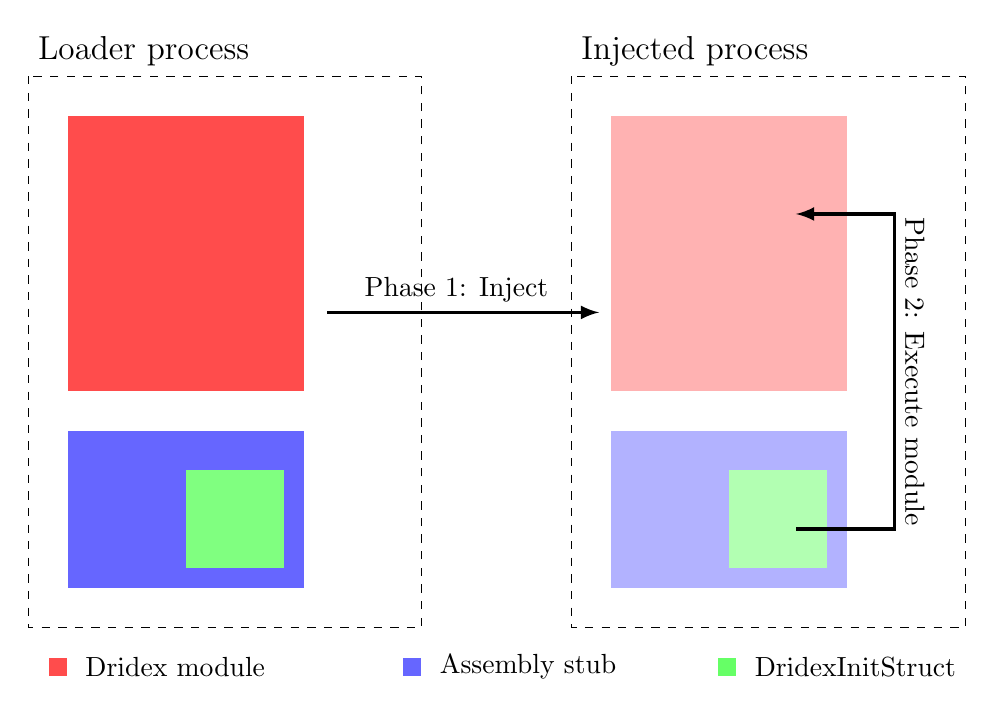
\begin{tikzpicture}
        \begin{scope}
            \node[anchor=south west] at (0, 0) {\large Loader process};
            \draw[dashed] (0, 0) rectangle (5,-7);

            \fill[fill=red!70] (0.5, -0.5) rectangle (3.5,-4);

            \fill[fill=blue!60] (0.5, -4.5) rectangle (3.5,-6.5);

            \fill[fill=green!50] (2, -5) rectangle (3.25,-6.25);
        \end{scope}

        \begin{scope}[xshift=6.9cm]
            \node[anchor=south west] at (0, 0) {\large Injected process};
            \draw[dashed] (0, 0) rectangle (5,-7);
    
            \fill[fill=red!30] (0.5, -0.5) rectangle (3.5,-4);
    
            \fill[fill=blue!30] (0.5, -4.5) rectangle (3.5,-6.5);
            \fill[fill=green!30] (2, -5) rectangle (3.25,-6.25);
        \end{scope}

        \draw[->,>=latex,line width=1.25pt] (3.8, -3) -- node[above,pos=0.475]{Phase 1: Inject} (7.25, -3);
        \draw[<-,>=latex,line width=1.25pt] (9.75, -1.75) -- (11, -1.75) -- node[above,midway,sloped]{Phase 2: Execute module} (11, -5.75) -- (9.75, -5.75);

        \node[fill=red!70,anchor=east] (A) at (0.5, -7.5) {};
        \node[anchor=west,right=1.5ex] at (A) {Dridex module};
        
        \node[fill=blue!60,anchor=east] (A) at (5, -7.5) {};
        \node[anchor=west,right=1.5ex] at (A) {Assembly stub};

        \node[fill=green!60,anchor=east] (A) at (9, -7.5) {};
        \node[anchor=west,right=1.5ex] at (A) {DridexInitStruct};
    \end{tikzpicture}
    \caption{Module execution via assembly stub\label{fig:Flow::ModuleExecution}}
\end{figure}

\lstinline|DridexInitStruct| contains various information to control the execution of the module as well as addresses of various Windows \gls{api} functions used by the stub itself.
\autoref{tab:Struct::DridexInitStruct} highlights the most important fields of \lstinline|DridexInitStruct|.
The fields \lstinline|stubBaseAddress|, \lstinline|WinApiNames|, \lstinline|sizeModule| and \lstinline|ptrModule| are used by the stub during the custom \lstinline|LoadLibrary| implementation while \lstinline|threadId|, \lstinline|hModuleThread| and \lstinline|stubLoopCondition| can be manipulated by the module itself to manage control flow in the stub.

\begin{quote}
\textbf{Note:} As the byte layout for this struct is extremely important in bootstrapping module execution its complete definition can be found in the \autoref{lst:Types::DridexInitStruct_full}.
\end{quote}

\begin{table}[htb]
    \centering
    \makebox[\linewidth][c]{
        \begin{tabular}{rcrl}
            \toprule
            Offset  &
            Size    &
            Name    &
            Description \\
            \midrule

            \texttt{0x0000} &
            \texttt{0x04}   &
            stubBaseAddress &
            Base address of the stub \\

            \texttt{0x0004} &
            \texttt{0x04}   &
            magicNumber     &
            Must match \texttt{0x56473829} \\

            \texttt{0x0008} &
            \texttt{0xF4}   &
            winApiNames     &
            Names of various important Windows \glspl{api} \\

            \multicolumn{2}{c}{\vdots} & \multicolumn{2}{c}{\vdots} \\

            \texttt{0x0128} &
            \texttt{0x04}   &
            threadId        &
            Id of the Thread to launch \\

            \texttt{0x012C} &
            \texttt{0x04}   &
            sizeModule      &
            Size of the module \\

            \texttt{0x0130} &
            \texttt{0x04}   &
            ptrModule       &
            Pointer to the module allocation \\

            \texttt{0x0134} &
            \texttt{0x04}   &
            hModuleThread   &
            Handle of the started child thread \\

            \texttt{0x0138}   &
            \texttt{0x04}     &
            stubLoopCondition &
            Condition of the stub main loop \\

            \multicolumn{2}{c}{\vdots} & \multicolumn{2}{c}{\vdots} \\

            \bottomrule
        \end{tabular}
    }
    \caption{Important fields of \lstinline|DridexInitStruct|\label{tab:Struct::DridexInitStruct}}
\end{table}

As calling \lstinline|DllMain| blocks the executing thread, the module starts a sub thread to carry out the desired task and saves a handle to it in \lstinline|DridexInitStruct.hModuleThread|.
Hereby the field \lstinline|DridexInitStruct.threadId| instructs the module which functionality should be executed.
The loader always initializes this field with 0 but the module can change it to schedule itself to be re executed with a different value.
The stub then waits on the module thread via the usual Windows \gls{api} function \lstinline|WaitForSingleObject|.
After the thread exits, the module is unloaded and the stub checks \lstinline|DridexInitStruct.stubLoopCondition| whether the module should be reloaded.
This mechanism permits a module to re-execute itself multiple times inside the same process.
\autoref{lst:Pseudo::Stub_ExecuteModule} shows this main loop of the assembly stub in pseudo code.
\\

\begin{lstlisting}[style=pseudo, caption={Module execution loop in assembler stub}, label={lst:Pseudo::Stub_ExecuteModule}]
// Stub_ExecuteModule(DridexInitStruct)
// Continuously execute a module by loading and freeing
%*\textbf{Stub\_ExecuteModule(\rmfamily\textit{i})}*
    ModuleSetup(%*\rmfamily\textit{i}*)
    DO
        LoadLibraryCustom(%*\rmfamily\textit{i}*, %*\rmfamily\textit{i.ptrPayload}*)
        WaitForSingleObject(%*\rmfamily\textit{i.hModuleThread}*, %*\rmfamily\textit{INFINITE}*)
        FreeLibraryCustom(%*\rmfamily\textit{i}*, %*\rmfamily\textit{i.ptrPayload}*)
    WHILE (%*\rmfamily\textit{i.stubLoopCondition}* %*\(\neq\)* 0)
    ModuleTearDown(%*\rmfamily\textit{i}*)
\end{lstlisting}

\vspace{1em}
So far, we described the first two stages in a Dridex infection as well as the module execution across user processes.
The next section contains our findings about the main bot module responsible for \gls{bn} communication as well as data exfiltration to the \gls{c2} as well as detailed protocol description on byte-level.

\section{\Gls{bot} stage\label{sec:Reverse_engineering_Dridex::Bot_stage}}
The \gls{bot} stage is entered after the loader executes the main \gls{bot} module via the assembler stub.
This stage pursues two main goals: Establish a connection to the \gls{bn} and register a new infected host as well as prepare the machine to steal data and credentials.

\subsection{Overview\label{subsec:Reverse_engineering_Dridex::Bot_stage::Overview}}
The main \gls{bot} module is structured into multiple threads with distinct functionalities.
While each main thread can and often does start other helper threads to perform background work, generally only one of the main threads is active at a time.
The \lstinline|DllMain| of the main \gls{bot} module performs some checks, on the filename of the executable in particular, verifies \lstinline|DridexInitStruct.magicNumber| and then launches a thread based on the value in \lstinline|DridexInitStruct.threadId|.
The possible values are described below as well as the corresponding functionality.

\begin{table}[htb]
    \centering
    \begin{tabular}{rl}
        \toprule
        \lstinline|threadId| &
        Functionality\\
        \midrule

        0 &
        Startup \& Initialization\\

        1 &
        \Gls{bn} communication\\

        2 &
        Browser hooking (Internet Explorer, Firefox \& Chrome)\\

        %2.2 &
        %Browser hooking (Google Chrome) \\

        %2.3 &
        %Browser hooking (Mozilla Firefox) \\

        3, 5 &
        Application hooking (via \lstinline|TranslateMessage| \& \lstinline|GetClipboardData|)\\

        4 &
        Synchronization logic\\

        6 &
        Generic Windows \gls{api} hooking of \lstinline|MessageBoxIndirectW|\\
        \bottomrule
    \end{tabular}
    \caption{Main \gls{bot} module threads\label{tab:Main_module::Threads}}
\end{table}

\begin{description}
    \item[Startup \& Initialization] This is the initial thread started by the launcher through the assembly stub.
    It enumerates the user processes and injects each suitable one with the module and an appropriate \lstinline|threadId|.
    One factor for the decision which id is selected, is the CRC32 of the executable name used to detect browser processes.
    The value gets computed for the process to inject and compared with a set of known constants for common browsers (shown in \autoref{tab:Main_module::BrowserCRC32}).
    If a match is found, the process is selected for \lstinline|threadId| \textbf{2} and injected.
    Further details about this decision process as well as the exact injection routines were out of scope of this thesis.
    \item[\Gls{bn} communication] The second thread is responsible for the complete \gls{bn} communication.
    When the initialization thread is finished it re-executes itself through the assembly stub with id \textbf{1} (cf:~\autoref{lst:Pseudo::Stub_ExecuteModule}) inside the supervision process.
    It starts multiple threads in the background to handle the different communication protocols and register itself to the \gls{c2}.
    One sub-thread in particular opens, binds, and listens on a socket accepting the \emph{\gls{p2p} protocol} used between bot and L2 node.
    We observed that the handler function for this socket is able to respond to a certain message which is only send to L2 nodes.
    This indicates that the node functionality is embedded into the main bot module and the bot is effectively able to act as a L2 node without being instructed by the \gls{c2}.
    \item[Browser hooking] This thread is responsible for hooking browser \glspl{api}.
    It hooks the relevant functions for the specific browser to intercept requests and responses to steal credentials according to the configuration.
    It can therefore be seen as the most important thread in regards to data collection on the infected machine.
    Details of the internal data structures storing the gathered data as well as the actual hooks were not part of the conducted analysis.
    \item[Application hooking] Threads \textbf{3} and \textbf{5} hook \lstinline|TranslateMessage| and \lstinline|GetClipboardData| and contain code to take screenshots to harvest data from the user.
    It remains unclear what condition triggers injection of these \lstinline|threadId|s as well as the exact differences between them.
    \item[Synchronization logic] The thread with id \textbf{4} seems to be responsible for synchronization between the multiple components.
    It uses \lstinline|WaitForMultipleObjects| and \lstinline|ReleaseMutex| on certain named synchronization primitives to ensure proper resource management.
    As this functionality was more related to the internal workings of Dridex it was not further analyzed.
    \item[Generic Windows \gls{api} hooking] The last thread seems to be tailored to programs using the Windows \gls{api} \lstinline|MessageBoxIndirectW| to collect sensitive information from the user.
    It hooks this function to collect and store this information for later exfiltration to the \gls{c2}.
\end{description}

\begin{table}
    \centering
    \begin{tabular}{rcl}
        \toprule
        Executable name &
        CRC32 &
        Browser \\
        \midrule

        ``firefox.exe'' &
        \texttt{0xB4E35F10} &
        Mozilla Firefox \\

        ``iexplore.exe''  &
        \texttt{0xC3DDC6D5} &
        Microsoft Internet Explorer \\

        ``chrome.exe'' &
        \texttt{0x9C1D0D0E} &
        Google Chrome \\
        \bottomrule
    \end{tabular}
    \caption[CRC32 of browser executables]{CRC32 of browser executables Dridex is able to hook\label{tab:Main_module::BrowserCRC32}}
\end{table}

\subsection{Protocols\label{subsec:Reverse_engineering_Dridex::Bot_stage::Protocols}}
The main bot module uses multiple protocols to communicate with differend endpoints.
The communication with the \gls{bm} is performed through the \emph{\gls{c2} protocol} while messages messages between bots and L2 nodes rely on the \emph{\gls{p2p} protocol}.

\begin{description}
    \item[\gls{c2} protocol] This protocol is mainly used for data exfiltration or confirmation of \gls{sp} elevation of new \glspl{bot}.
    Messages are encrypted with the \gls{c2}'s public key which is embedded in the main \gls{bot} module itself and signed with a generated RSA private key that is transmitted to the \gls{c2} as part of the registration process.
    As this protocol is more complex and not tremendously useful in determining whether a host is infected, it is not focus of this thesis.
    However it should be studied in future research to potentially be able to detect when stolen data is exfiltrated from a host.
    \item[\gls{p2p} protocol] The \gls{p2p} protocol is mainly used for messages that are uninteresting for the \gls{c2} including configuration and \gls{pl} update messages which are cached by the second and third layer~(cf:~\autoref{fig:Dridex::Network_layers}).
    It is synchronously transmitted over raw \acrshort{tcp} sockets and uses RC4 for on-the-wire obfuscation.
    This means that one side (usually the \gls{bot}) initiates a connection to another peer on the advertised port, sends a request message and receives a response on the same socket.
    The connection is terminated afterwards even if the message exchange results in a new connection attempt from the \gls{bot}.
    Interestingly, messages can be directly decrypted on the wire, as the ephemeral keys for the encryption are directly embedded into the message.
\end{description}

The routine responsible for binding the listening socket for the \gls{p2p} protocol follows a specific algorithm to decide which port number is used.
As shown in \autoref{lst:BindPortForP2P} the algorithm first checks whether the port number of a previous successful run is stored.
If the variable is set and can be bound it is immediately chosen und and the routine returns.
This mechanism looks like a crash recovery routine in case the thread responsible for botnet communication exited abnormally as \lstinline|portToBind| was never set initially when the malware starts.
Next an external string containing port numbers divided by a semicolon is checked for valid entries, results enumerated and again the first available port is chosen.
The string was never even allocated in our test runs and as such the purpose of it remains currently unknown.
If no viable port is found up to this point a list of hardcoded numbers (stored in \lstinline|.rdata|) is enumerated and checked for availability.
This list includes the ports for \gls{http} and \gls{https} as well as popular fallback variants of the two which is likely an attempt to deceive misconfigured firewalls and hide behind regular traffic.
It is important to note that the ports are always enumerated in the order shown in \autoref{lst:BindPortForP2P}.
This fact in combination with the early return style makes ports at the end of the list a lot less likely to be used.
If this also does not result in a useable socket the algorithm falls back to enumerating all ports from \lstinline|1000| to \texttt|65000|.
\\

\begin{lstlisting}[style=pseudo, caption={\gls{p2p} protocol: port selection algorithm}, label={lst:BindPortForP2P}]
CONST PREFERRED_PORTS = [443, 8443, 3443, 4443, 444, 448, 843, 943, 1443, 80, 8080, 8000, 8888]
GLOBAL %*\rmfamily\textit{portToBind}*, %*\rmfamily\textit{portsString}*
// BindPortForP2P
// Select and bind an available port for the p2p protocol
%*\textbf{BindPortForP2P()}*
    IF %*\rmfamily\textit{portToBind}* %*\(\neq\)* 0 AND CanBindPort(%*\rmfamily\textit{portToBind}*)
        RETURN BindPort(%*\rmfamily\textit{portToBind}*)

    FOR %*\rmfamily\textit{port}* %*\(\in\)* GetPortsFromString(%*\rmfamily\textit{portsString, ";"}*)
        IF CanBindPort(%*\rmfamily\textit{port}*)
            %*\rmfamily\textit{portToBind} \(\gets\) \rmfamily\textit{port}*
            RETURN BindPort(%*\rmfamily\textit{port}*)

    FOR %*\rmfamily\textit{port}* %*\(\in\)* PREFERRED_PORTS
        IF CanBindPort(%*\rmfamily\textit{port}*)
            %*\rmfamily\textit{portToBind} \(\gets\) \rmfamily\textit{p}*
            RETURN BindPort(%*\rmfamily\textit{port}*)

    FOR %*\rmfamily\textit{port}* %*\(\in\) \(\{x \in \mathbb{N} \mid 1000 \leq x \leq 65000\}\)*
        IF CanBindPort(%*\rmfamily\textit{port}*)
            %*\rmfamily\textit{portToBind} \(\gets\) \rmfamily\textit{p}*
            RETURN BindPort(%*\rmfamily\textit{port}*)
\end{lstlisting}

\begin{figure}
    \centering
    \begin{bytefield}[bitwidth=\linewidth/10]{8}
        \bitheader{0-7} \\
        \begin{leftwordgroup}{Header}
            \wordbox{3}{Random header\\ \(\langle~128~\text{bytes}~\rangle\)} \\
        \begin{rightwordgroup}{Payload}
            \bitbox[bl]{4}{Payload length} & \bitbox[lr]{4}{}
        \end{leftwordgroup} \\
            \wordbox[lr]{1}{RC4 key for message length} \\
            \bitbox[bl]{4}{} & \bitbox{4}{Encrypted message length} \\
            \wordbox[blr]{2}{RC4 key for message} \\
            \wordbox[lrb]{3}{(RC4) \textbf{Encrypted message}\\ (GZip stream with zeroed timestamp)\\ \(\langle~\cdots~\rangle\)}
        \end{rightwordgroup} \\
    \end{bytefield}
    \caption{\gls{p2p} protocol: envelope layout\label{bf:P2P::Envelope}}
\end{figure}

\autoref{bf:P2P::Envelope} shows the \emph{envelope} of a message in the \emph{\gls{p2p} protocol}.
Each passed message is wrapped in this fashion to obscure the message's content in a potential traffic flow analysis.
The envelope can be divided into \emph{header} and \emph{payload} sections.
\begin{description}
    \item[Header] The first 128 bytes of the header consist of 32 integers which when added result in 0.
    These bytes are used to increase the difficulty of detecting \gls{p2p} messages in network traffic and serve no further purpose; the \gls{mw} verifies and discards these bytes.
    A validation failure of these integers results in a complete drop of the message.
    In addition the header contains the length of the payload which is encoded in two signed \lstinline|short|s.
    The encoding algorithm is shown in \autoref{lst:Pseudo::EncodePayloadLength} and further described in~\cite[p.~9-10]{anubisnetworks2015dridex}.
    As the \gls{p2p} protocol is transmitted over raw \gls{tcp} sockets, this size is required to know how many more bytes should be read.
    \item[Payload] The payload consists of two randomly generated 16-byte RC4 keys and the encrypted message as well as its encrypted length.
    The first key is used to encrypt the following length while the second key encrypts the message.
    This encryption layer is not preventing on-the-fly decryption as the keys are directly present in the envelope.
    Its main goal is to obfuscate the Gzip header of the message which could easily be detected by its magic numbers.
    Furthermore, Dridex zeroes out the timestamp of the Gzip stream making it even easier to identify by pattern based \glspl{ids}.
\end{description}
\vspace{1em}

\begin{lstlisting}[style=pseudo, caption={Payload length encoding}, label={lst:Pseudo::EncodePayloadLength}]
// EncodePayloadLength(len)
// Store a payload length integer in two signed shorts
%*\textbf{EncodePayloadLength(\rmfamily\textit{len})}*
    %*\rmfamily\textit{high} \(\gets\) \rmfamily\textit{len / 30000}*
    %*\rmfamily\textit{low} \(\gets\) \rmfamily\textit{len \% 30000}*
    %*\rmfamily\textit{highBytes} \(\gets\) *Reverse(%*\rmfamily\textit{high}*)
    %*\rmfamily\textit{lowBytes} \(\gets\) *Reverse(%*\rmfamily\textit{high}*)
    RETURN %*\rmfamily\textit{highBytes} + \rmfamily\textit{lowBytes}*
\end{lstlisting}

The actual message format after unzipping differs between requests and responses; \autoref{bf:P2P::Request} shows the mandatory fields of a request.
The first byte represents the \emph{length} of the two following \emph{RC4 key parts}.
Each one of the parts is \lstinline|length| bytes long and when xored they result in the RC4 key for this message exchange.
The next byte is the \emph{request type} which dictates how the rest of the message is interpreted.
An overview of the possible request types is given in \autoref{tab:Main_module::P2P::RequestTypesAndCodes}.
The last mandatory field of the message is an the encrypted \emph{BotId} of the sender which is again encoded in the common string encoding as previously in the loader request (cf:~\autoref{bf:Loader::Request}).
This field is mandatory even if the handler functions for certain request types do not use it.
Depending on the request type more fields might be appended.

\begin{figure}
    \centering
    \begin{bytefield}[bitwidth=\linewidth/9]{8}
        \bitheader{0-7} \\
        \bitbox{1}{Length} & \bitbox[rt]{7}{} \\
        \wordbox[lr]{1}{RC4 Key\\ \(\langle~2*\text{\texttt{length} bytes}~\rangle\)} \\
        \wordbox[blr]{1}{} \\
        \bitbox[lrb]{1}{\let\bw=\width\ \vspace{1em}\resizebox{\bw}{!}{\,\textbf{request type}\,}} & \bitbox[rt]{7}{} \\
        \wordbox[blr]{3}{(RC4) Encrypted \textbf{BotId}\\ \(\langle~\cdots~\rangle\)} \\
    \end{bytefield}
    \caption{\gls{p2p} protocol: request message layout\label{bf:P2P::Request}}
\end{figure}

The request type dictates how the message is interpreted and indicates the receiver what action the sender wants to initiate.
\autoref{tab:Main_module::P2P::RequestTypesAndCodes} lists the request types found in the analyzed sample.
The request types 0 and 1 both perform an unknown calculation on the BotId of the sender and compare the result with internal state.
Additionally the handling routine for type 1 loops through internal state representing the known (or possibly installed) modules of this \gls{bot}.
It is assumed that these two request types represent \gls{sp} endpoints related to \gls{pl} and binary updates but that theory could not be verified in the scope of this thesis.
We focussed our efforts towards request type 2, which categorizes messages related to the \emph{CheckMe} process, because it contains messages very suitable for scanning and crawling.
These messages also contain a \emph{request code} as the first field to further distinguish between the multiple requests involved.
The \emph{CheckMe} process will be described in greater detail later on in this chapter.

\begin{table}
    \centering
    \begin{tabular}{rcl}
        \toprule
        Request type &
        Request code &
        Description \\
        \midrule

        \texttt{0} &
        --- &
        Related to \gls{pl}/membership management \\

        \texttt{1}  &
        --- &
        Same as 0 but also send module information \\
        \midrule

        \texttt{2} &
        \texttt{100/0x64} &
        CheckMe: `\lstinline|checkme|'\\

        \texttt{2} &
        \texttt{101/0x65} &
        CheckMe: `\lstinline|ping|' \\

        \texttt{2} &
        \texttt{102/0x66} &
        Unknown: Contains second \gls{p2p} payload \\
        \bottomrule
    \end{tabular}
    \caption{\gls{p2p} protocol: request types \& codes\label{tab:Main_module::P2P::RequestTypesAndCodes}}
\end{table}

The format of responses is highly dependant on the request type and has no mandatory fields.
Responses related to the \emph{CheckMe} process always start with an encrypted \emph{\gls{ascii} status code} similar to the ones from \gls{http}.
These status codes are always 4 byte long and consist of the \gls{ascii} characters of the status code prefixed with \lstinline|0x30|/``\lstinline|0|''.
All further fields are optional and are usually encrypted with the RC4 key provided in the request.
Examples layouts for responses will be given later on this chapter.

\begin{figure}
    \centering
    \makebox[\linewidth][c]{
        \begin{tikzpicture}[thick,node distance=7cm,auto,>=stealth']
            % Define and draw nodes
            \node[] (bot) {\large \Gls{bot}};
            \node[right of=bot] (l2) {\large Layer 2 node};
            \node[right of=l2, node distance=6cm] (c2) {\large Dridex \gls{c2}};
            \node[below of=bot, node distance=6cm] (bot_ground) {};
            \node[below of=l2, node distance=6cm] (l2_ground) {};
            \node[below of=c2, node distance=6cm] (c2_ground) {};

            % Draw node lines
            \draw (bot) -- (bot_ground);
            \draw (l2) -- (l2_ground);
            \draw (c2) -- (c2_ground);

            % Draw lines
            \draw[->, draw=teal] ($(bot)!0.25!(bot_ground)$) -- node[above,midway]{`\textcolor{blue}{\texttt{checkme}}' request (including \textcolor{darkred}{port})} ($(l2)!0.25!(l2_ground)$);

            \draw[<-, draw=darkred] ($(bot)!0.45!(bot_ground)$) -- node[above,midway]{`\textcolor{blue}{\texttt{ping}}' request on specified \textcolor{darkred}{port}} ($(l2)!0.45!(l2_ground)$);
            \draw[->, dashed, draw=darkred] ($(bot)!0.55!(bot_ground)$) -- node[below,midway]{`\textcolor{blue}{\texttt{pong}}' response} ($(l2)!0.55!(l2_ground)$);

            \draw[->, dashed] ($(l2)!0.65!(l2_ground)$) -- node[above,midway]{``new L2 candidate''} ($(c2)!0.65!(c2_ground)$);
            \draw[<-, dashed] ($(l2)!0.75!(l2_ground)$) -- node[below,midway]{``L2 confirmed? (y/n)''} ($(c2)!0.75!(c2_ground)$);

            \draw[<-, draw=teal] ($(bot)!0.85!(bot_ground)$) -- node[below,midway]{`\textcolor{blue}{\texttt{checkme\_result}}' response} ($(l2)!0.85!(l2_ground)$);
        \end{tikzpicture}
    }
    \caption{\gls{p2p} Communication flow in \emph{CheckMe} phase\label{fig:Communication::Bot_stage::Checkme}}
\end{figure}

As mentioned above the \emph{CheckMe} process is especially interesting to detect infected hosts.
This process is initiated by the \gls{bot} in thread 1 after the listening socket has been opened.
The goal is to detect whether the \gls{bot}'s \acrshort{ip} address is reachable from the open Internet making it a possible \gls{sp}/L2 node.
\autoref{fig:Communication::Bot_stage::Checkme} gives an overview over the communication flow. 
The \gls{bot} starts the process by sending a `\lstinline|checkme|' request to an L2 node (shown in~\autoref{bf:P2P::Request::Checkme}).
This message contains the request code \lstinline|0x64|/\lstinline|100| and the port the \gls{bot} previously selected to handle to the \gls{p2p} protocol.

\begin{figure}
    \vspace{2em}
    \centering
    \begin{bytefield}[bitwidth=\linewidth/10]{8}
        \bitheader{0-7} \\
        \wordbox{2}{\gls{p2p} request message (request type 2, cf:~\autoref{bf:P2P::Request})\\ \(\langle~\cdots~\rangle\)} \\
        \bitbox[blr]{1}{\texttt{0x64}} & \bitbox[blr]{2}{\textbf{\gls{p2p} port}} \\
    \end{bytefield}
    \caption{\gls{p2p} protocol: `\lstinline|checkme|' request\label{bf:P2P::Request::Checkme}}
\end{figure}

\begin{figure}
    \vspace{2em}
    \centering
    \begin{bytefield}[bitwidth=\linewidth/10]{8}
        \bitheader{0-7} \\
        \wordbox{2}{\gls{p2p} request message (request type 2, cf:~\autoref{bf:P2P::Request})\\ \(\langle~\cdots~\rangle\)} \\
        \bitbox[blr]{1}{\texttt{0x65}} \\
    \end{bytefield}
    \caption{\gls{p2p} protocol: `\lstinline|ping|' request\label{bf:P2P::Request::Ping}}
\end{figure}

The node then opens a connection to the \gls{bot} on this port and tries to send a `\lstinline|ping|' request.
As depicted in \autoref{bf:P2P::Request::Ping} this message only contains the request code \lstinline|0x65|/\lstinline|101|.
This connection can only succeed if the receiving \gls{bot} has a public \gls{ip} address as the inbound connection would be filtered by a \gls{nat} device or firewall.
If this request succeeds and is correctly handled by the \gls{bot} it would be a possible \gls{sp} and as such very interesting for the Dridex \gls{bm}.  

The expected response to this request is the `\lstinline|pong|' message which follows the layout shown in \autoref{bf:P2P::Response::Pong}.
As this message belongs to the \emph{CheckMe} process, the first field is an encrypted status code: \lstinline|0x504F4E47|/``\lstinline|PONG|''.
Additionally, the peer responding to the `\lstinline|ping|' request appends its own BotId (again encrypted with the RC4 key from this request).

\begin{figure}
    \centering
    \begin{bytefield}[bitwidth=\linewidth/10]{8}
        \bitheader{0-7} \\
        \bitbox{4}{(RC4) Encrypted \texttt{``PONG''}} & \bitbox[rt]{4}{} \\
        \wordbox[blr]{3}{(RC4) Encrypted BotId (sender)\\ \(\langle~\cdots~\rangle\)} \\
    \end{bytefield}
    \caption{\gls{p2p} protocol: `\lstinline|pong|' response\label{bf:P2P::Response::Pong}}
\end{figure}

\begin{figure}
    \vspace{2em}
    \centering
    \begin{bytefield}[bitwidth=\linewidth/10]{4}
        \bitheader{0-3} \\
        \bitbox{4}{(RC4) Encrypted \textbf{status code}} \\
    \end{bytefield}
    \caption{\gls{p2p} protocol: `\lstinline|checkme_result|' response\label{bf:P2P::Response::Checkme_result}}
\end{figure}

The layout of the `\lstinline|checkme_result|' response is detailed in \autoref{bf:P2P::Response::Checkme_result}; it consists of only a single status code integer.
In case of a failure during the `\lstinline|ping|' request ``\lstinline|0404|'' is returned.
If the message exchange was completed successfully the \gls{c2} decides whether the new host should be included in \glspl{pl} based on the new \gls{bot}'s id and \gls{ip} address.
``\lstinline|0200|'' informs the \gls{bot} that it is now a L2 node, while ``\lstinline|0503|'' signals a rejection by the \gls{c2}.
It is unclear whether a \gls{bot} can be elevated to an L2 node at a later time.

We now have a good understanding about the \gls{p2p} protocol used by Dridex and especially the \emph{CheckMe} process.
This information will later be used to efficiently detect active \glspl{sp}.


\section{Obfuscation measures\label{sec:Reverse_engineering_Dridex::Obfuscation_measures}}
Besides the complicated module execution process, Dridex employs a diverse array of obfuscation measures to impede security analysis.
Besides standard practices like packing and encryption Windows \gls{api} functions are dynamically resolved both in the loader and the main bot module.
Furthermore a novel code injection technique is used to prevent automated detection by \glspl{sandbox}.

\subsection{Packing\label{subsec:Reverse_engineering_Dridex::Obfuscation_measures::Packing}}
Both the loader and the main module are protected by an unknown---possible custom-made---protector (cf:~\autoref{sec:Related_work::Anti_reverse_engineering_techniques}), which modifies the loaded binary image in-place before transferring control to the actual entry point of the \gls{mw}. \autoref{fig:MemoryLayout::Protector} shows the memory layout during the unpacking process as well as the control flow.
First a large memory segment is allocated, filled with the decrypted unpacking routines and consequently invoked.
The unpacker then marks the entire memory region containing the binary image as writable and proceeds to unpack its content in-place.
Finally the function directly jumps back to the binary's original entry-point address which now points to the decrypted instructions.

\begin{figure}
    \begin{tikzpicture}
        \begin{scope}
            \node[anchor=south west] at (0, 0) {\hspace{-0.5em}\large Binary image};
            \draw[dashed, fill=blue!50] (0, 0) rectangle (3.5,-4);
        \end{scope}

        \begin{scope}[xshift=7.75cm]
            \node[anchor=south west] at (0, 0) {\hspace{-0.5em}\large Unpacker segment};
            \draw[dashed,fill=red!50] (0, 0) rectangle (3.5,-4);
            \draw[dashed,pattern=crosshatch dots, pattern color=red!40!black] (0, 0) rectangle (3.5,-4);
        \end{scope}

        \draw[->,>=latex,line width=1.25pt,dashed] (1.75, -4.25) -- node[above,pos=0.475]{} (1.75, -5.75);

        \begin{scope}[yshift=-6cm]
            \draw[dashed, fill=blue!50] (0, 0) rectangle (3.5, -4);
            \fill[yellow!80!black] (0, -0.5) rectangle (3.5, -0.75);
            \fill[green!60!black] (0, -0.75) rectangle (3.5, -1.25);
            \fill[blue!70] (0, -1.25) rectangle (3.5, -1.75);
            \fill[yellow!80!black] (0, -1.75) rectangle (3.5, -2.5);
            \fill[green!60!black] (0, -2.5) rectangle (3.5, -3);
            \fill[blue!70] (0, -3) rectangle (3.5, -3.25);
            \fill[blue!40] (0, -3.25) rectangle (3.5, -4);
            \draw[dashed, pattern=crosshatch dots, pattern color=blue!40!black] (0, 0) rectangle (3.5, -4);
        \end{scope}


        \draw[->,>=latex,line width=1.25pt] (3, -1) -- node[above,pos=0.5]{1. Allocate + decrypt} (8.25, -1);
        \draw[->,>=latex,line width=1.25pt] (3, -2) -- node[above,pos=0.45]{2. Transfer control} (8.25, -2);
        \draw[->,>=latex,line width=1.25pt] (8.25, -3.25) -- node[above,pos=0.51,sloped]{3. Change protection} (3.75, -6);
        \draw (8.25, -3.25) -- node[below,pos=0.55,sloped]{4. Unpack in-place} (3.75, -6);
        \draw[->,>=latex,line width=1.25pt] (9.5, -3.25) -- (9.5, -8) -- node[above,midway,sloped]{5. Re-execute entry-point} (3.75, -8);
        \node[pattern=crosshatch dots,pattern color=red!40!black,anchor=east,minimum size=0.5cm] (A) at (5, -9.5) { };

        \node[anchor=west,right=7ex,pattern=crosshatch dots,pattern color=blue!40!black,anchor=east,minimum size=0.5cm] (B) at (A) {};
        \node[anchor=west,right=3ex] at (B) {Writable memory};
    \end{tikzpicture}
    \caption{Protector: Memory layout \& control flow\label{fig:MemoryLayout::Protector}}
\end{figure}

The protector used by Dridex is characterized by large amounts of seemingly \emph{dead code} and \emph{fake Windows API calls}.
The dead code---often computation on integer constants which had no apparent use---can be explained by the fact, that the packer unpacks in-place.
The large amount of \lstinline|mov| and \lstinline|add|/\lstinline|sub| instructions are simply placeholders to reserve enough space in the binary image to store the resulting machine code.
In addition, they confuse inexperienced reverse engineers by burying them in useless instructions so that the few important ones (such as control flow decisions and memory allocation) might stay undetected.

The Windows \gls{api} calls are carefully placed behind \emph{fake conditional jumps} to distract further from the real malicious purpose.
These instructions such as \lstinline|jle| (``Jump Less Equal'') and \lstinline|jz| (``Jump (if) Zero'') are usually used to control execution flow based on a previous calculation.
In the packed versions of the loader as well as the bot module these calculations were indeed locally independent and based off constants effectively placing the \gls{api} calls in unreachable code.
\autoref{lst:ASM::Unreachable} shows an example for this kind of obfuscation; both \lstinline[style=asm]|edx| and \lstinline[style=asm]|ebx| are initialized from constants, then modified by other operations with other constants and finally compare placing \lstinline|call_imported_win_api| in unreachable code.
\\

\begin{lstlisting}[style=asm, caption={Example: Unreachable Windows \gls{api} calls}, label={lst:ASM::Unreachable}]
mov edx, 0x12345678
mov ebx, 0x87654321
    %*\smash{\vdots}*
add ebx, 0x43215678
sub edx, ebx
    %*\smash{\vdots}*
cmp ebx, edx              ; result is constant
jnz call_imported_win_api ; this jump is never taken
    %*\smash{\vdots}*                     ; continue loader routine
\end{lstlisting}

While a regular packer can usually be sufficiently defeated by manual unpacking in a debugger, we encountered several problems when dumping the unpacked payload.
Although the base packing routine was quickly identified and circumvented---by carefully placing breakpoints at the end of the unpacking routine and dumping the unpacked sections via \lstinline|ProcessDump|\fnote{\url{https://github.com/glmcdona/Process-Dump}}---the resulting binary contained several small errors (similar to bitflips).
This sometimes resulted in straight-up invalid instructions and othertimes incorrect \lstinline|call| or \lstinline|jmp| offsets.
After performing multiple iterations of dumping the unpacked binary, multiple binaries were obtained which all had different invalid sections enabling us to continually patch the initial version by diffing them with each unpacked module.
Unfortunately, this delayed the analysis at times because the errors often went undetected for extended periods of time since the functions were just not called and the recovery process required sometimes multiple dumps because the error was also present in the first new one taken.
The variation could be attributed to randomization (which is used in packers to hide their existence) but since the resulting binaries produced a segmentation fault in the affected areas this seems unlikely.
Ultimately the reason for this behavior remains unknown and may indicate either a bug in the (un-)packer or be the result of another hidden anti-reverse engineering measure.

\subsection{Atom Bombing\label{subsec:Reverse_engineering_Dridex::Obfuscation_measures::Atom_Bombing}}
Starting from version 4 Dridex started to use an innovative memory injection technique called \emph{Atom Bombing}.
The traditional approach to copy malicious payloads into other processes involved several Windows \glspl{api} for managing virtual memory which are rarely used in regular legitimate programs.
First the \gls{mw} would allocate memory in the target process via \lstinline|VirtualAlloc|, write a malicious payload to that allocation with a call to \lstinline|WriteProcessMemory|, mark it as executable via \lstinline|VirtualProtect| and finally transfer control to the payload via \lstinline|CreateRemoteThread|.
Although alternatives exist for all three functions, these \gls{api} calls can easily monitored by anti-virus software making them unattractive to \gls{mw} developers.

Atom Bombing instead uses \emph{atom tables}, a feature of Windows, in combination with \gls{apc} to achieve memory injection without relying on the above \glspl{api}.
These atom tables store null-terminated strings identified by a unique key on the \gls{os} level making them available to all processes in the system.
Dridex leverages that feature to encode its own binary code in the atom table and uses \lstinline|NtQueueAPCThread| to retrieve the data inside a thread of the target process.
It then simply marks the memory region as executable by calling \lstinline|VirtualProtect| and executes the payload again through an \gls{apc} thread.
While the execution permission could have also been achieved through Atom Bombing this process is significantly harder and the Dridex developers opted to just call the known \gls{api} for simplicity.
Since the main injection was achieved without calling the usual functions the adoption of this concept required \glspl{sandbox} to extend their list of monitored Windows \glspl{api}.

During the dissection of the \gls{mw} we found the code related to Atom Bombing in both the loader and the main bot module indicating that this process is now Dridex's memory injection technique of choice.
However, as the this topic was not the focus of this thesis it was not further analyzed or documented.
For detailed descriptions of the technical details we refer to the blog post by the team which discovered the technique~\cite{liberman2016atombombing}.


\subsection{Encrypted data\label{subsec:Reverse_engineering_Dridex::Obfuscation_measures::Encrypted_data}}
To further protect critical information after the packer has been circumvented, Dridex encrypts several areas in both the loader as well as the main bot binary.
These areas are usually stored in the standard section for read-only memory in \gls{pe} binaries: \lstinline|.rdata| and contain multiple related entries.
Decryption is performed by the function \lstinline|DridexCrypt| which expects an index argument and uses RC4 in combination with a custom indexing routine to return the requested data.
\lstinline|DridexCrypt| is also used in other places where RC4 is required such as \gls{p2p} protocol handling; in this case the index is omitted.

Dridex encrypts the following static information:
\begin{itemize}
    \item (Parts of) registry keys
    \item (Parts of) file names
    \item Log format strings
    \item Protocol keywords
    \item Assembly stubs used in Atom Bombing and module execution
\end{itemize}

When analyzing the decryption routine we found it to be also very self contained which made it relatively easy to mass decrypt entire areas at once with a simple Python script.
The script directly manipulates registers such as \lstinline|eip| or \lstinline|ecx| during debug execution through IDA's \gls{api} and calls \lstinline|DridexCrypt| repeatedly on the same encrypted section until all data has been exhausted.

\subsection{Dynamic API calls\label{subsec:Reverse_engineering_Dridex::Obfuscation_measures::Dynamic_API_calls}}
All calls to the Windows \gls{api} beginning from the loader are hidden behind a resolver function \lstinline|WinAPIFromHash|.
This function takes two hashes of both the \gls{dll}, which contains the method to call, and the function name and returns the address of the function while also loading known system \gls{dll} if they have not been mapped into the process' address space yet.

This prevents disassemblers to automatically infer the function signature and aid in the analysis.
In regular library calls (through the \gls{pe} Import Table) tools like IDA Pro can resolve the function and match it with internal definitions to infer characteristics like calling convention, argument and return types.
This information helps to quickly identify types of stack variables and also allows the reverse engineer to quickly find all calls to a specific function via cross-references.

\begin{figure}
    \centering
    \makebox[\linewidth][c]{
        \begin{subfigure}[b]{0.35\textwidth}
            \includegraphics[width=\linewidth]{img/function_call_regular}
            \caption{Regular Windows \gls{api} call}
        \end{subfigure}
        \begin{subfigure}[b]{0.678\textwidth}
            \includegraphics[width=\linewidth]{img/function_call_obfuscated}
            \caption{Obfuscated Windows \gls{api} call}
        \end{subfigure}
    }
    \caption{Windows \gls{api} call obfuscation through \texttt{WinAPIFromHash\label{fig:Windows_API_call_obfuscation}}}
\end{figure}

\autoref{fig:Windows_API_call_obfuscation} demonstrates the difference between a regular imported function call and Dridex's \lstinline|WinAPIFromHash|.
In the standard case, IDA is able to identify the arguments pushed to the stack and add their names to the respective instructions as comments.
Furthermore, they are also properly typed as well as renamed to match the function signature which helps immensely in deciphering the function's purpose.
In contrast, the result of the call to \lstinline|WinAPIFromHash| cannot be statically determined which leaves IDA unable to correctly process the function's arguments.

To overcome this obfuscation layer the python script \lstinline|tag_hashes.py| was written. 
It uses the IDA's Python \gls{api} to find immediate values which look like \gls{dll} or function name hashes and performs a lookup in a set of known values.
If a match is found the script adds a comment to the specific instruction in the IDA database while unknown values are printed with their offset in the binary.
This enables the reverse engineer to iteratively resolve single hashes, add them to the script's knowledge base and rerun the script to annotate all occurrences of the newly found function.

Luckily \lstinline|WinAPIFromHash| is highly self contained and does not require any special setup besides the hashes passed in the standard registers for the \lstinline|fastcall| calling convention, \lstinline|ecx| and \lstinline|edx|.
This permits the reverse engineer to jump through the function's cross-references, selectively load the hashes into the registers and call the function to quickly decode hashes.

\begin{figure}
    \centering
    \includegraphics[width=.75\textwidth]{img/memory_annotation_dynamic}
    \caption{Dynamic memory annotations in IDA Pro\label{fig:IDA::Memory_annotation}}
\end{figure}

As shown in \autoref{fig:IDA::Memory_annotation} IDA annotates all uses of named memory locations directly even when they are loaded or calculated dynamically during runtime.
In addition the used notation \lstinline|<binary_without_extension>_<function_name>| can be double clicked to jump to the address if it is currently mapped in the address space.
Therefore, the annotations produced by \lstinline|tag_hashes.py| can be used to quickly navigate to the resolved function if desired.


\section{Summary\label{sec:Reverse_engineering_Dridex::Summary}}
We have now described the Dridex infection process and its most important stages.
The loader uses simple RC4 encryption with an hard-coded key to communicate with the distribution server and is used to download the malicious modules and an initial L2 node \gls{pl}.
The request messages for this process were documented on the byte-level.
Next the modules are injected in multiple processes and executed through an embedded assembly stub.
The execution mechanism inside the stub including its core structure were introduced and detailed in pseudo code.

The main bot module itself is divided into multiple discrete threads which are selected based on the process the module was injected into.
Common targets for injection are browsers which the \gls{mw} is able to hook to extract sensitive information.
We described the roles of each thread with a focus on the one responsible for \gls{bn} communication.
Finally, a comprehensive summary of the \emph{CheckMe} process concludes the chapter.
Next to a conceptual description we also provided message layout figures and detailed important \emph{request types} and \emph{response status codes}.

With the information presented in this chapter we are now prepared to implement the Dridex L2 scanner to verify the correctness of the protocol descriptions.